\chapter{Navier--Stokes 方程组:不可压缩流动的数学模型}\label{chap:navier-stokes}\label{chap:flow-equations}

\begin{note}[基本原理和变量]\label{note:basic-principles}
流体力学的基本方程称为 Navier--Stokes 方程组.对于等温流动(isothermal flow),也就是温度保持恒定的流动,它表达两条物理守恒定律:质量守恒(conservation of mass)和线动量守恒(conservation of linear momentum).推导这些方程有多种方法.这里概述连续介质力学(continuum mechanics)中的经典推导;这种方法包含若干启发式步骤.

流动由以下变量描述:
\begin{itemize}
  \item $\rho(t,\bm{x})$:密度,单位为 $\mathrm{kg}/\mathrm{m}^3$;
  \item $\bm{v}(t,\bm{x})$:速度,单位为 $\mathrm{m}/\mathrm{s}$;
  \item $P(t,\bm{x})$:压力,单位为 $\mathrm{Pa}=\mathrm{N}/\mathrm{m}^2$.
\end{itemize}
假设这些函数在时间区间 $[0,T]$ 和区域 $\Omega\subset\mathbb{R}^3$ 上具有足够的光滑性.
\end{note}

\section{质量守恒}\label{sec:mass-conservation}
\markright{\thesection\ 质量守恒}

\begin{note}[一般守恒律]\label{note:general-conservation-law}
取 $\Omega$ 中任意一个固定不动的开体积区域 $\Omega$,假设其边界 $\partial\Omega$ 足够光滑.区域 $\Omega$ 内的质量为
\begin{equation*}
  m(t)=\int_{\Omega}\rho(t,\bm{x})\,\mathrm{d}\bm{x}\quad[\mathrm{kg}].
\end{equation*}
如果 $\Omega$ 内的质量守恒,那么区域内质量的变化率必须等于穿过 $\Omega$ 边界的质量通量(mass flux).质量通量为 $\rho\bm{v}(t,\bm{x})$,单位是 $\mathrm{kg}/(\mathrm{m}^2\mathrm{s})$,因此
\begin{equation}\label{eq:mass-balance-integral}
  \frac{\mathrm{d}}{\mathrm{d}t}m(t)
  =\frac{\mathrm{d}}{\mathrm{d}t}\int_{\Omega}\rho(t,\bm{x})\,\mathrm{d}\bm{x}
  =-\int_{\partial\Omega}\rho(t,\bm{s})\,\bm{v}(t,\bm{s})\cdot\bm{n}(\bm{s})\,\mathrm{d}s.
\end{equation}
这里 $\bm{n}(\bm{s})$ 是边界上指向外侧的单位法向量.
\end{note}

假设所有函数以及 $\partial\Omega$ 都足够光滑,就可以应用散度定理(divergence theorem,即分部积分公式):
\begin{equation*}
  \int_{\Omega}\nabla\cdot(\rho\bm{v})(t,\bm{x})\,\mathrm{d}\bm{x}
  =\int_{\partial\Omega}(\rho\bm{v})(t,\bm{s})\cdot\bm{n}(\bm{s})\,\mathrm{d}s.
\end{equation*}
将这一恒等式代入\cref{eq:mass-balance-integral},并交换对时间的微分与对空间的积分,得到
\begin{equation*}
  \int_{\Omega}\bigl(\partial_t\rho(t,\bm{x})+
    \nabla\cdot(\rho\bm{v})(t,\bm{x})\bigr)\,\mathrm{d}\bm{x}=0.
\end{equation*}
由于 $\Omega$ 是任意选取的体积区域,必有
\begin{equation}\label{eq:continuity-equation}
  \partial_t\rho+\nabla\cdot(\rho\bm{v})=0,
  \qquad 0<t<T,\quad\bm{x}\in\Omega.
\end{equation}
这就是流体力学的第一条方程,称为连续性方程.

\begin{note}[随时间变化的区域]\label{note:time-dependent-domain}
也可以考虑随时间变化的区域 $\Omega(t)$.此时可以应用 Reynolds 输运定理(Reynolds transport theorem).设 $\eta(t,\bm{x})$ 是定义在任意区域 $\Omega(t)$ 上且足够光滑的函数,区域边界 $\partial\Omega(t)$ 也足够光滑,则 Reynolds 输运定理为
\begin{equation}\label{eq:reynolds-transport}
  \frac{\mathrm{d}}{\mathrm{d}t}\int_{\Omega(t)}\eta(t,\bm{x})\,\mathrm{d}\bm{x}
  =\int_{\Omega(t)}\partial_t\eta(t,\bm{x})\,\mathrm{d}\bm{x}
   +\int_{\partial\Omega(t)}\eta(t,\bm{s})\,\bm{v}(t,\bm{s})\cdot\bm{n}(\bm{s})\,\mathrm{d}s.
\end{equation}
\end{note}

在 $\eta(t,\bm{x})$ 取为密度的特殊情形下,区域内质量的变化率为
\begin{equation*}
  \frac{\mathrm{d}}{\mathrm{d}t}\int_{\Omega(t)}\rho(t,\bm{x})\,\mathrm{d}\bm{x}
  =\int_{\Omega(t)}\partial_t\rho(t,\bm{x})\,\mathrm{d}\bm{x}
   +\int_{\partial\Omega(t)}\rho(t,\bm{s})\,\bm{v}(t,\bm{s})\cdot\bm{n}(\bm{s})\,\mathrm{d}s.
\end{equation*}
由质量守恒和散度定理可得
\begin{equation*}
  0=\int_{\Omega(t)}\bigl(\partial_t\rho+\nabla\cdot(\rho\bm{v})\bigr)(t,\bm{x})\,\mathrm{d}\bm{x}.
\end{equation*}
由于 $\Omega(t)$ 任意,\cref{eq:continuity-equation} 仍然成立.

\begin{note}[不可压缩均质流体]\label{note:incompressible-homogeneous}
如果流体不可压缩且均质,也就是只由一种流体组成,那么 $\rho(t,\bm{x})=\rho>0$ 为常数,\cref{eq:continuity-equation} 化为
\begin{equation}\label{eq:divergence-free}
  \partial_x v_1+\partial_y v_2+\partial_z v_3
  =\nabla\cdot\bm{v}=0,
  \qquad 0<t<T,\quad\bm{x}\in\Omega.
\end{equation}
其中
\begin{equation*}
  \bm{v}(t,\bm{x})=
  \begin{pmatrix}v_1(t,\bm{x})\\v_2(t,\bm{x})\\v_3(t,\bm{x})\end{pmatrix}.
\end{equation*}
因此,对于不可压缩均质流体,质量守恒只对速度施加约束.
\end{note}

\section{线动量守恒}\label{sec:momentum-conservation}
\markright{\thesection\ 线动量守恒}

\begin{note}[牛顿第二运动定律]\label{note:newton-second-law}
线动量守恒是牛顿第二运动定律
\begin{equation}\label{eq:newton-second-law}
  \text{合力}=\text{质量}\times\text{加速度}
\end{equation}
在流动问题中的表达.它指出,一群流体质点的线动量变化率必须等于作用在这群质点上的合力.
\end{note}

\begin{note}[线动量守恒]\label{note:momentum-conservation}
任意区域 $\Omega$ 内的线动量为
\begin{equation*}
  \int_{\Omega}\rho\bm{v}(t,\bm{x})\,\mathrm{d}\bm{x}
  \quad[\mathrm{N}\,\mathrm{s}].
\end{equation*}
因此,可以仿照\cref{note:general-conservation-law},将区域 $\Omega$ 内的线动量守恒写成
\begin{equation*}
  \frac{\mathrm{d}}{\mathrm{d}t}\int_{\Omega}\rho\bm{v}(t,\bm{x})\,\mathrm{d}\bm{x}
  =-\int_{\partial\Omega}\rho\bm{v}(\bm{v}\cdot\bm{n})(t,\bm{s})\,\mathrm{d}s
    +\int_{\Omega}\bm{f}^{\mathrm{net}}(t,\bm{x})\,\mathrm{d}\bm{x}
  \quad[\mathrm{N}],
\end{equation*}
左端表示区域内动量的变化,右端第一项表示动量穿过 $\Omega$ 边界的通量,$\bm{f}^{\mathrm{net}}$ 是区域内的合力密度,单位为 $\mathrm{N}/\mathrm{m}^3$.其中
\begin{equation*}
  \bm{v}(\bm{v}\cdot\bm{n})
  =\begin{pmatrix}
    v_1v_1n_1+v_1v_2n_2+v_1v_3n_3\\
    v_2v_1n_1+v_2v_2n_2+v_2v_3n_3\\
    v_3v_1n_1+v_3v_2n_2+v_3v_3n_3
  \end{pmatrix}
  =\bm{v}\bm{v}^{\top}\bm{n}.
\end{equation*}
应用分部积分,并交换对时间的微分与对区域 $\Omega$ 的积分,可得
\begin{equation*}
  \int_{\Omega}\Bigl(\partial_t(\rho\bm{v})
    +\nabla\cdot(\rho\bm{v}\bm{v}^{\top})\Bigr)(t,\bm{x})\,\mathrm{d}\bm{x}
  =\int_{\Omega}\bm{f}^{\mathrm{net}}(t,\bm{x})\,\mathrm{d}\bm{x}.
\end{equation*}
乘积法则给出
\begin{equation}\label{eq:momentum-product-rule}
\begin{aligned}
  \int_{\Omega}\Bigl(&\partial_t\rho\,\bm{v}+\rho\,\partial_t\bm{v}
      +\bm{v}\bm{v}^{\top}\nabla\rho
      +\rho(\nabla\cdot\bm{v})\bm{v}
      +\rho(\bm{v}\cdot\nabla)\bm{v}\Bigr)(t,\bm{x})\,\mathrm{d}\bm{x}\\
  &=\int_{\Omega}\bm{f}^{\mathrm{net}}(t,\bm{x})\,\mathrm{d}\bm{x}.
\end{aligned}
\end{equation}
在通常的记号 $(\bm{v}\cdot\nabla)\bm{v}$ 中,可以把 $\bm{v}\cdot\nabla$ 理解为算子
\begin{equation*}
  \bm{v}\cdot\nabla=v_1\partial_x+v_2\partial_y+v_3\partial_z,
\end{equation*}
它分别作用于 $\bm{v}$ 的每个分量.文献中也常把 $(\bm{v}\cdot\nabla)\bm{v}$ 写成 $\bm{v}\cdot\nabla\bm{v}$.

对于不可压缩流动,$\rho$ 为常数,且已知 $\nabla\cdot\bm{v}=0$,见\cref{eq:divergence-free};因此,\cref{eq:momentum-product-rule} 化为
\begin{equation*}
  \int_{\Omega}\rho\Bigl(\partial_t\bm{v}
    +(\bm{v}\cdot\nabla)\bm{v}\Bigr)(t,\bm{x})\,\mathrm{d}\bm{x}
  =\int_{\Omega}\bm{f}^{\mathrm{net}}(t,\bm{x})\,\mathrm{d}\bm{x}.
\end{equation*}
由于 $\Omega$ 是任意选取的区域,可得守恒定律
\begin{equation*}
  \rho\Bigl(\partial_t\bm{v}+(\bm{v}\cdot\nabla)\bm{v}\Bigr)
  =\bm{f}^{\mathrm{net}},
  \qquad 0<t<T,\quad\bm{x}\in\Omega.
\end{equation*}
利用\cref{eq:reynolds-transport},也可以对随时间变化的区域 $\Omega(t)$ 推导出同一守恒定律.
\end{note}

\begin{note}[外力]\label{note:external-forces}
作用在 $\Omega$ 上的力包括外力(体力)和内力.外力例如重力、浮力,以及电磁力(在液态金属中).这些力汇总为体力项
\begin{equation*}
  \int_{\Omega}\bm{f}^{\mathrm{ext}}(t,\bm{x})\,\mathrm{d}\bm{x}.
\end{equation*}
\end{note}

\begin{note}[内力、Cauchy 原理与应力张量]\label{note:internal-forces-stress}
内力是流体对自身施加的力,包括压力,以及一个“流体微元”对相邻微元施加的黏性阻力.内力属于接触力,也就是说,它们作用在流体微元 $\Omega$ 的表面上.令 $\bm{t}\,[\mathrm{N}/\mathrm{m}^2]$ 表示这种内力向量,它称为 Cauchy 应力向量(Cauchy stress vector)或牵引向量(traction vector),则作用在 $\Omega$ 上的内力为
\begin{equation*}
  \int_{\partial\Omega}\bm{t}(t,\bm{s})\,\mathrm{d}s.
\end{equation*}
于是,对任意固定不随时间变化的区域 $\Omega$,线动量守恒方程为
\begin{equation}\label{eq:momentum-balance-with-tractions}
\begin{aligned}
  \int_{\Omega}\rho(t,\bm{x})
    \Bigl(\partial_t\bm{v}+(\bm{v}\cdot\nabla)\bm{v}\Bigr)(t,\bm{x})\,\mathrm{d}\bm{x}
  ={}&\int_{\Omega}\bm{f}^{\mathrm{ext}}(t,\bm{x})\,\mathrm{d}\bm{x}\\
    &+\int_{\partial\Omega}\bm{t}(t,\bm{s})\,\mathrm{d}s.
\end{aligned}
\end{equation}

\cref{eq:momentum-balance-with-tractions} 右端表示作用于区域 $\Omega$ 内部及其边界的合力.接下来需要详细描述其中的内力,也就是 $\bm{t}(t,\bm{s})$ 所表示的力.

连续介质力学以 Cauchy 应力原理为基础.Cauchy 对内接触力的设想是:在 $\partial\Omega$ 上任意一个(假想的)平面,都存在一个力;从几何角度看,该力只依赖于平面的取向.因此,$\bm{t}=\bm{t}(\bm{n})$,其中 $\bm{n}$ 是该假想平面指向外侧的单位法向量.

下面说明 $\bm{t}$ 关于 $\bm{n}$ 呈线性依赖.为此,考虑一个四面体区域 $\Omega$,其顶点为
\begin{equation*}
\begin{aligned}
  \bm{p}_0&=(0,0,0)^{\top},\qquad
  \bm{p}_1=(x_1,0,0)^{\top},\\
  \bm{p}_2&=(0,y_2,0)^{\top},\qquad
  \bm{p}_3=(0,0,z_3)^{\top},\\
  &x_1,y_2,z_3>0.
\end{aligned}
\end{equation*}
见\cref{fig:tetrahedron}.包含 $\bm{p}_1,\bm{p}_2,\bm{p}_3$ 的平面记作 $\partial\Omega_{(\bm{n})}$.其指向外侧的单位法向量为
\begin{equation}\label{eq:tetrahedron-normal}
\begin{aligned}
  \bm{n}
  &=\frac{(\bm{p}_2-\bm{p}_1)\times(\bm{p}_3-\bm{p}_1)}
        {\lVert(\bm{p}_2-\bm{p}_1)\times(\bm{p}_3-\bm{p}_1)\rVert_2}\\
  &=\frac{1}{\lVert(\bm{p}_2-\bm{p}_1)\times(\bm{p}_3-\bm{p}_1)\rVert_2}
      \begin{pmatrix}y_2z_3\\z_3x_1\\x_1y_2\end{pmatrix}
   =\begin{pmatrix}n_1\\n_2\\n_3\end{pmatrix}.
\end{aligned}
\end{equation}
法向量为 $-\bm{e}_i$ 的四面体面记作 $\partial\Omega_{(\bm{e}_i)}$,其中 $i=1,2,3$.令 $\bm{t}(\bm{n})$ 表示作用在 $\partial\Omega_{(\bm{n})}$ 上的 Cauchy 应力向量.假设 Cauchy 应力向量只依赖相应表面的法向量,那么它在四面体的每个面上都是常向量,各面的积分便可直接计算.

\begin{elegantfigure}[0.514\paperwidth]
  \includegraphics[page=23,pagebox=cropbox,trim=106.50bp 97.40bp 107.36bp 356.25bp,clip,width=\linewidth]{../input/source/Finite Element Methods for Incompressible Flow Problems.pdf}
  \captionof{figure}{用于讨论 Cauchy 应力向量关于法向量线性依赖关系的四面体示意图.}\label{fig:tetrahedron}
\end{elegantfigure}

\cref{eq:newton-second-law} 和四面体体积公式给出
\begin{equation}\label{eq:traction-force-balance}
  \bm{t}(\bm{n})\,|\partial\Omega_{(\bm{n})}|
  -\sum_{i=1}^{3}\bm{t}(\bm{e}_i)\,|\partial\Omega_{(\bm{e}_i)}|
  =-\frac{h(\bm{n})}{3}\,|\partial\Omega_{(\bm{n})}|\,\bm{a},
  \qquad[\mathrm{N}],
\end{equation}
其中 $|\cdot|$ 表示相应面的面积,$\bm{t}(\bm{e}_i)$ 是面 $\partial\Omega_{(\bm{e}_i)}$ 上的常应力向量,$\bm{a}$ 是加速度,单位为 $\mathrm{m}/\mathrm{s}^2$;$h(\bm{n})$ 表示面 $\partial\Omega_{(\bm{n})}$ 到原点的距离.利用叉积可计算 $\partial\Omega_{(\bm{n})}$ 的面积:
\begin{equation*}
  |\partial\Omega_{(\bm{n})}|
  =\frac{1}{2}\bigl|(\bm{p}_2-\bm{p}_1)\times(\bm{p}_3-\bm{p}_1)\bigr|_2
  =\frac{1}{2}\left|\begin{pmatrix}y_2z_3\\z_3x_1\\x_1y_2\end{pmatrix}\right|_2.
\end{equation*}
利用\cref{eq:tetrahedron-normal} 对法向量的表示,可以得到
\begin{equation*}
  |\partial\Omega_{(\bm{e}_1)}|
  =\frac{1}{2}y_2z_3
  =\frac{1}{2}n_1\bigl|(\bm{p}_2-\bm{p}_1)\times(\bm{p}_3-\bm{p}_1)\bigr|_2
  =|\partial\Omega_{(\bm{n})}|\,n_1.
\end{equation*}
对 $|\partial\Omega_{(\bm{e}_2)}|$ 和 $|\partial\Omega_{(\bm{e}_3)}|$ 也可得到类似公式.将这些公式代入\cref{eq:traction-force-balance},可得
\begin{equation}\label{eq:traction-normal-limit}
  \bm{t}(\bm{n})-\sum_{i=1}^{3}\bm{t}(\bm{e}_i)n_i
  =-\frac{h(\bm{n})}{3}\,\bm{a}.
\end{equation}
现在令四面体收缩至原点,同时令 $\partial\Omega_{(\bm{n})}$ 沿 $\bm{n}$ 的方向移动.此时\cref{eq:traction-normal-limit} 左端保持不变,而由于 $h(\bm{n})\to0$,右端趋于零.因此,取极限可得
\begin{equation*}
  \bm{t}(\bm{n})
  =\sum_{i=1}^{3}\bm{t}(\bm{e}_i)n_i
  =\begin{pmatrix}\bm{t}(\bm{e}_1)&\bm{t}(\bm{e}_2)&\bm{t}(\bm{e}_3)\end{pmatrix}\bm{n}.
\end{equation*}
这里最后一个矩阵的各列分别为对应的向量.这个关系表明,$\bm{t}(\bm{n})$ 关于 $\bm{n}$ 线性依赖.

因此,Cauchy 应力向量的模型为
\begin{equation}\label{eq:cauchy-stress-model}
  \bm{t}=\bm{S}\bm{n},
\end{equation}
其中 $\bm{S}(t,\bm{x})\,[\mathrm{N}/\mathrm{m}^2]$ 是一个 $3\times3$ 张量,称为应力张量(stress tensor).应力张量表示流动中的全部内力.将\cref{eq:cauchy-stress-model} 代入\cref{eq:momentum-balance-with-tractions} 中表示内力的边界积分,并应用散度定理,得到
\begin{equation*}
  \int_{\partial\Omega}\bm{t}(t,\bm{s})\,\mathrm{d}s
  =\int_{\Omega}\nabla\cdot\bm{S}(t,\bm{x})\,\mathrm{d}\bm{x},
\end{equation*}
这里张量散度按行定义:
\begin{equation*}
  \nabla\cdot\bm{A}
  =\begin{pmatrix}
    \partial_x a_{11}+\partial_y a_{12}+\partial_z a_{13}\\
    \partial_x a_{21}+\partial_y a_{22}+\partial_z a_{23}\\
    \partial_x a_{31}+\partial_y a_{32}+\partial_z a_{33}
  \end{pmatrix}.
\end{equation*}
由于\cref{eq:momentum-balance-with-tractions} 对任意区域 $\Omega$ 都成立,因而
\begin{equation}\label{eq:momentum-equation}
  \rho\Bigl(\partial_t\bm{v}+(\bm{v}\cdot\nabla)\bm{v}\Bigr)
  =\nabla\cdot\bm{S}+\bm{f}^{\mathrm{ext}},
  \qquad 0<t<T,\quad\bm{x}\in\Omega.
\end{equation}
这就是动量方程.
\end{note}

\begin{note}[应力张量的对称性]\label{note:stress-symmetry}
取边界 $\partial\Omega$ 足够光滑的任意区域 $\Omega$,并令合力由\cref{eq:momentum-balance-with-tractions} 右端给出.关于坐标原点 $\bm{0}$ 的力矩(torque)定义为
\begin{equation}\label{eq:torque}
  \bm{M}_0
  =\int_{\Omega}\bm{r}\times\bm{f}^{\mathrm{ext}}\,\mathrm{d}\bm{x}
   +\int_{\partial\Omega}\bm{r}\times(\bm{S}\bm{n})\,\mathrm{d}s
  \quad[\mathrm{N}\,\mathrm{m}],
\end{equation}
这里使用了\cref{eq:cauchy-stress-model},且 $\bm{r}=x\bm{e}_1+y\bm{e}_2+z\bm{e}_3$ 是从原点指向点 $\bm{x}\in\Omega$ 的向量.直接计算可得
\begin{equation*}
  \bm{r}\times(\bm{S}\bm{n})
  =\bigl(\bm{r}\times\bm{S}_{*1}\quad
         \bm{r}\times\bm{S}_{*2}\quad
         \bm{r}\times\bm{S}_{*3}\bigr)\bm{n},
\end{equation*}
其中 $\bm{S}_{*i}$ 表示 $\bm{S}$ 的第 $i$ 列.将此式代入\cref{eq:torque},应用分部积分并使用乘积法则,得到
\begin{equation}\label{eq:torque-volume-form}
\begin{aligned}
  \bm{M}_0
  ={}&\int_{\Omega}\bm{r}\times\bm{f}^{\mathrm{ext}}\,\mathrm{d}\bm{x}
    +\int_{\Omega}\bm{r}\times(\nabla\cdot\bm{S})\,\mathrm{d}\bm{x}\\
   &+\int_{\Omega}\bigl(\partial_x\bm{r}\times\bm{S}_{*1}
       +\partial_y\bm{r}\times\bm{S}_{*2}
       +\partial_z\bm{r}\times\bm{S}_{*3}\bigr)\,\mathrm{d}\bm{x}.
\end{aligned}
\end{equation}
现在考虑处于平衡状态的流体,即作用在流体上的合力为零.于是,\cref{eq:momentum-equation} 右端为零,\cref{eq:torque-volume-form} 的前两个积分之和也为零.此外,平衡还要求 $\bm{M}_0=\bm{0}$.因此,\cref{eq:torque-volume-form} 给出
\begin{equation}\label{eq:stress-symmetry-derivatives}
  \bm{0}=\int_{\Omega}\bigl(\partial_x\bm{r}\times\bm{S}_{*1}
       +\partial_y\bm{r}\times\bm{S}_{*2}
       +\partial_z\bm{r}\times\bm{S}_{*3}\bigr)\,\mathrm{d}\bm{x}.
\end{equation}
由
\begin{equation*}
  \partial_x\bm{r}
  =\lim_{\Delta x\to0}
    \frac{(x+\Delta x)\bm{e}_1-x\bm{e}_1}{\Delta x}
  =\bm{e}_1,
\end{equation*}
以及 $\partial_y\bm{r}=\bm{e}_2$、$\partial_z\bm{r}=\bm{e}_3$,将这些等式代入\cref{eq:stress-symmetry-derivatives},最终得到
\begin{equation*}
  \bm{0}=\int_{\Omega}
  \begin{pmatrix}
    S_{32}-S_{23}\\S_{13}-S_{31}\\S_{21}-S_{12}
  \end{pmatrix}(t,\bm{x})\,\mathrm{d}\bm{x}.
\end{equation*}
该式对任意区域 $\Omega$ 都成立,因此应力张量必为对称张量,即 $\bm{S}=\bm{S}^{\top}$,且只有六个未知分量.
\end{note}

\begin{note}[应力张量的分解]\label{note:stress-decomposition}
为了用\cref{note:basic-principles} 中引入的基本变量建立应力张量模型,将它分解为
\begin{equation}\label{eq:stress-decomposition}
  \bm{S}=\bm{V}-P\bm{I}.
\end{equation}
这里 $\bm{V}\,[\mathrm{N}/\mathrm{m}^2]$ 是黏性应力张量(viscous stress tensor),表示由粒子间摩擦产生的力;$P\,[\mathrm{Pa}]$ 是压力,描述作用在每个流体体积 $\Omega$ 表面上的力;$\bm{I}$ 为单位张量.黏性应力张量将用速度来建模,见\cref{note:viscous-stress}.
\end{note}

\begin{note}[压力]\label{note:pressure}
压力 $P$ 作用于流体体积 $\Omega$ 的表面时,方向总是垂直于表面并指向 $\Omega$ 内部.\cref{eq:stress-decomposition} 中的负号正体现了这一性质,因为
\begin{equation*}
  -\int_{\partial\Omega}P\bm{n}\,\mathrm{d}s
  =-\int_{\Omega}\nabla P\,\mathrm{d}\bm{x}
  =-\int_{\Omega}\nabla\cdot(P\bm{I})\,\mathrm{d}\bm{x}.
\end{equation*}
\end{note}

\begin{note}[黏性应力张量]\label{note:viscous-stress}
只有流体粒子以不同速度运动时,粒子之间才会产生摩擦.因此,黏性应力张量建模为速度梯度的函数.为保证对称性(见\cref{note:stress-symmetry}),它取决于速度梯度的对称部分,即速度形变率张量(velocity rate-of-deformation tensor),简称速度形变张量:
\begin{equation*}
  \bm{D}(\bm{v})
  =\frac{\nabla\bm{v}+(\nabla\bm{v})^{\top}}{2}
  \quad[1/\mathrm{s}].
\end{equation*}
速度梯度是一个张量,其分量为
\begin{equation*}
  (\nabla\bm{v})_{ij}=\partial_jv_i
  =\frac{\partial v_i}{\partial x_j},
  \qquad i,j=1,2,3.
\end{equation*}

如果速度梯度不太大,可以假设这种依赖关系首先是线性的,其次可以忽略高阶导数.对于速度为常数的流动,速度梯度为零,也不会产生摩擦;因此,模型中不应出现速度一阶导数以外的低阶项.满足上述全部条件的张量最一般形式为
\begin{equation*}
  \bm{V}=a\bm{D}(\bm{v})+b(\nabla\cdot\bm{v})\bm{I},
\end{equation*}
其中 $a$ 和 $b$ 不依赖于速度.引入一阶黏度 $\mu\,[\mathrm{kg}/(\mathrm{m}\,\mathrm{s})]$ 和二阶黏度 $\zeta\,[\mathrm{kg}/(\mathrm{m}\,\mathrm{s})]$ 后,流体力学中将该张量写为
\begin{equation}\label{eq:viscous-stress-law}
  \bm{V}=2\mu\bm{D}(\bm{v})
    +\left(\zeta-\frac{2\mu}{3}\right)
      (\nabla\cdot\bm{v})\bm{I}
  \quad[\mathrm{N}/\mathrm{m}^2].
\end{equation}
黏度 $\mu$ 也称为动力黏度(dynamic viscosity)或剪切黏度(shear viscosity).对于流体,\cref{eq:viscous-stress-law} 与固体的 Hooke 定律相对应.
\end{note}

\begin{example}[稳态旋转]\label{ex:steady-rotation}
流体作稳态旋转时,不存在黏性应力,即 $\bm{V}=\bm{0}$.此时速度为
\begin{equation*}
  \bm{v}=\symbf{\Omega}\times\bm{x}
  =\begin{pmatrix}\Omega_1\\\Omega_2\\\Omega_3\end{pmatrix}
   \times\begin{pmatrix}x\\y\\z\end{pmatrix}
  =\begin{pmatrix}
    \Omega_3y-\Omega_2z\\
    \Omega_1z-\Omega_3x\\
    \Omega_2x-\Omega_1y
  \end{pmatrix},
\end{equation*}
其中 $\symbf{\Omega}\,[1/\mathrm{s}]$ 为常角速度(angular velocity).显然,$\nabla\cdot\bm{v}=0$,并且
\begin{equation*}
  \nabla\bm{v}=
  \begin{pmatrix}
    0&\Omega_3&-\Omega_2\\
    -\Omega_3&0&\Omega_1\\
    \Omega_2&-\Omega_1&0
  \end{pmatrix}
  \quad\Longrightarrow\quad
  \bm{D}(\bm{v})=\bm{0}.
\end{equation*}
因此,\cref{eq:viscous-stress-law} 在这种情形下是合适的模型.
\end{example}

\begin{note}[Newton 型流体]\label{note:newtonian-fluid}
线性关系\cref{eq:viscous-stress-law} 只是对真实流体的一种近似.一般而言,这种关系是非线性的;只有在应力较小时,才能对一般的应力--形变关系作线性近似.线性应力--形变关系由 Newton 提出,因此满足\cref{eq:viscous-stress-law} 假设的流体称为 Newton 型流体(Newtonian fluid).还存在比\cref{eq:viscous-stress-law} 更一般的关系,不过从数学角度看,对它们的理解还不够充分.
\end{note}

\begin{note}[法向应力、剪切应力与应力张量的迹]\label{note:stress-trace}
应力张量 $\bm{S}$ 的对角分量 $S_{11},S_{22},S_{33}$ 称为法向应力,非对角分量称为剪切应力.对于不可压缩流动,由\cref{eq:divergence-free,eq:stress-decomposition,eq:viscous-stress-law} 可得
\begin{equation}\label{eq:incompressible-stress}
  \bm{S}=2\mu\bm{D}(\bm{v})-P\bm{I}.
\end{equation}
应力张量的迹是法向应力之和:
\begin{equation*}
\begin{aligned}
  \operatorname{tr}(\bm{S})
  &=S_{11}+S_{22}+S_{33}\\
  &=2\mu(\partial_xv_1+\partial_yv_2+\partial_zv_3)
    +3\left(\zeta-\frac{2\mu}{3}\right)(\nabla\cdot\bm{v})-3P\\
  &=3\zeta(\nabla\cdot\bm{v})-3P.
\end{aligned}
\end{equation*}
对于不可压缩流体,因而有
\begin{equation*}
  \operatorname{tr}(\bm{D}(\bm{v}))
  =\frac{1}{2\mu}\bigl(\operatorname{tr}(\bm{S})
       +\operatorname{tr}(P\bm{I})\bigr)
  =\frac{1}{2\mu}(-3P+3P)=0,
\end{equation*}
并且
\begin{equation}\label{eq:pressure-from-stress-trace}
  P(t,\bm{x})=-\frac{1}{3}
    (S_{11}+S_{22}+S_{33})(t,\bm{x}).
\end{equation}
\end{note}

\begin{note}[Navier--Stokes 方程组]\label{note:full-navier-stokes}
现在将应力张量中的压力部分和黏性应力张量模型\cref{eq:viscous-stress-law} 代入\cref{eq:momentum-equation},得到包含质量守恒方程在内的一般 Navier--Stokes 方程组:
\begin{equation}\label{eq:general-navier-stokes}
\begin{aligned}
  &\rho\bigl(\partial_t\bm{v}
        +(\bm{v}\cdot\nabla)\bm{v}\bigr)
   -2\nabla\cdot\bigl(\mu\bm{D}(\bm{v})\bigr)\\
  &\quad-\nabla\cdot\left(
      \left(\zeta-\frac{2\mu}{3}\right)
      (\nabla\cdot\bm{v})\bm{I}\right)
      +\nabla P=\bm{f}^{\mathrm{ext}},\\
  &\partial_t\rho+\nabla\cdot(\rho\bm{v})=0,
  \qquad (t,\bm{x})\in(0,T)\times\Omega.
\end{aligned}
\end{equation}
如果流体不可压缩且均质,使得 $\mu$ 和 $\rho$ 为正的常数,Navier--Stokes 方程组可简化为
\begin{equation}\label{eq:incompressible-navier-stokes}
\begin{aligned}
  \partial_t\bm{v}-2\nu\nabla\cdot\bm{D}(\bm{v})
    +(\bm{v}\cdot\nabla)\bm{v}
    +\nabla\frac{P}{\rho}
  &=\frac{\bm{f}^{\mathrm{ext}}}{\rho},
  &&(t,\bm{x})\in(0,T)\times\Omega,\\
  \nabla\cdot\bm{v}&=0,
  &&(t,\bm{x})\in(0,T)\times\Omega.
\end{aligned}
\end{equation}
这里 $\nu=\mu/\rho\,[\mathrm{m}^2/\mathrm{s}]$ 是流体的运动黏度(kinematic viscosity).
\end{note}

\section{无量纲 Navier--Stokes 方程组}\label{sec:dimensionless-navier-stokes}
\markright{\thesection\ 无量纲方程}
\markright{\thesection}

\begin{note}[特征尺度]\label{note:characteristic-scales}
数学分析和数值模拟以无量纲方程(dimensionless equations)为基础.为了从\cref{eq:incompressible-navier-stokes} 导出无量纲方程,引入以下量:
\begin{itemize}
  \item $L\,[\mathrm{m}]$:流动问题的特征长度尺度(characteristic length scale);
  \item $U\,[\mathrm{m}/\mathrm{s}]$:流动问题的特征速度尺度(characteristic velocity scale);
  \item $T^*\,[\mathrm{s}]$:流动问题的特征时间尺度(characteristic time scale).
\end{itemize}
\end{note}

\begin{note}[无量纲 Navier--Stokes 方程组]\label{note:dimensionless-equations}
用 $(t',\bm{x}')\,[\mathrm{s},\mathrm{m}]$ 表示原变量.作变量变换
\begin{equation}\label{eq:dimensionless-variable-transform}
  \bm{x}=\frac{\bm{x}'}{L},\qquad
  \bm{u}=\frac{\bm{v}}{U},\qquad
  t=\frac{t'}{T^*}.
\end{equation}
由\cref{eq:incompressible-navier-stokes} 并经尺度变换,得到
\begin{equation*}
\begin{aligned}
  \frac{L}{UT^*}\partial_t\bm{u}
   -\frac{2\nu}{UL}\nabla\cdot\bm{D}(\bm{u})
   +(\bm{u}\cdot\nabla)\bm{u}
   +\nabla\frac{P}{\rho U^2}
  &=\frac{L}{\rho U^2}\bm{f}^{\mathrm{ext}},\\
  \nabla\cdot\bm{u}&=0.
\end{aligned}
\end{equation*}
这里所有导数都针对新变量.虽然记号中没有特别标出,区域和时间区间此时也都已无量纲化.定义
\begin{equation}\label{eq:dimensionless-parameters}
  p=\frac{P}{\rho U^2},\qquad
  \mathrm{Re}=\frac{UL}{\nu},\qquad
  \mathrm{St}=\frac{L}{UT^*},\qquad
  \bm{f}=\frac{L}{\rho U^2}\bm{f}^{\mathrm{ext}}.
\end{equation}
于是得到无量纲形式的不可压缩 Navier--Stokes 方程组:
\begin{equation}\label{eq:dimensionless-navier-stokes}
\begin{aligned}
  \mathrm{St}\,\partial_t\bm{u}
   -\frac{2}{\mathrm{Re}}\nabla\cdot\bm{D}(\bm{u})
   +(\bm{u}\cdot\nabla)\bm{u}+\nabla p
  &=\bm{f},
  &&(t,\bm{x})\in(0,T)\times\Omega,\\
  \nabla\cdot\bm{u}&=0,
  &&(t,\bm{x})\in(0,T)\times\Omega.
\end{aligned}
\end{equation}
常数 $\mathrm{Re}$ 称为 Reynolds 数(Reynolds number),常数 $\mathrm{St}$ 称为 Strouhal 数(Strouhal number).这两个数可用于对不同流动进行分类和比较.
\end{note}

\begin{note}[无量纲 Navier--Stokes 方程组的固有困难]\label{note:dimensionless-difficulties}
为了简化记号,取特征时间 $T^*=L/U$,于是\cref{eq:dimensionless-navier-stokes} 化为
\begin{equation}\label{eq:dimensionless-ns-standard}
\begin{aligned}
  \partial_t\bm{u}-2\nu\nabla\cdot\bm{D}(\bm{u})
    +(\bm{u}\cdot\nabla)\bm{u}+\nabla p
  &=\bm{f},
  &&(t,\bm{x})\in(0,T)\times\Omega,\\
  \nabla\cdot\bm{u}&=0,
  &&(t,\bm{x})\in(0,T)\times\Omega.
\end{aligned}
\end{equation}
这里无量纲黏度(dimensionless viscosity)$\nu=\mathrm{Re}^{-1}$.稍有滥用记号之处在于,此处沿用运动黏度的符号表示无量纲黏度.

上述变换以及由此得到的\cref{eq:dimensionless-ns-standard},是不可压缩 Navier--Stokes 方程数学分析和不可压缩流动数值模拟的基本方程.系统\cref{eq:dimensionless-ns-standard} 包含两个重要困难:
\begin{itemize}
  \item 速度与压力之间的耦合;
  \item 对流项的非线性.
\end{itemize}
此外,当对流项占主导、也就是 $\nu$ 很小时,数值模拟也会遇到困难.
\end{note}

\begin{note}[式 \texorpdfstring{(2.25)}{(2.25)} 中各项的不同形式]\label{note:equivalent-term-forms}
借助散度约束,即\cref{eq:dimensionless-ns-standard} 的第二个方程,可以对 Navier--Stokes 方程组中的黏性项和对流项作等价改写.

设 $\bm{u}$ 足够光滑且 $\nabla\cdot\bm{u}=0$.利用 Schwarz 定理(Schwarz theorem)和\cref{eq:dimensionless-ns-standard} 的第二个方程,直接计算可得
\begin{equation}\label{eq:viscous-laplacian-identity}
\begin{aligned}
  \nabla\cdot(\nabla\bm{u})&=\Delta\bm{u},\\
  \nabla\cdot\bigl((\nabla\bm{u})^{\top}\bigr)
  &=\nabla(\nabla\cdot\bm{u})
   =\begin{pmatrix}
     \partial_x(\nabla\cdot\bm{u})\\
     \partial_y(\nabla\cdot\bm{u})\\
     \partial_z(\nabla\cdot\bm{u})
    \end{pmatrix}
   =\bm{0}.
\end{aligned}
\end{equation}
因此,黏性项可以写成
\begin{equation}\label{eq:viscous-term-laplacian}
  -2\nu\nabla\cdot\bm{D}(\bm{u})=-\nu\Delta\bm{u}.
\end{equation}

对于对流项,利用下列恒等式(乘积法则):
{\small
\begin{equation}\label{eq:convective-product-rule}
\begin{aligned}
  \nabla\cdot(\bm{u}\bm{v}^{\top})
  & =\begin{pmatrix}
      \partial_x(u_1v_1)+\partial_y(u_1v_2)+\partial_z(u_1v_3)\\
      \partial_x(u_2v_1)+\partial_y(u_2v_2)+\partial_z(u_2v_3)\\
      \partial_x(u_3v_1)+\partial_y(u_3v_2)+\partial_z(u_3v_3)
     \end{pmatrix}\\
  & =\begin{pmatrix}
      u_1(\partial_xv_1+\partial_yv_2+\partial_zv_3)\\
      u_2(\partial_xv_1+\partial_yv_2+\partial_zv_3)\\
      u_3(\partial_xv_1+\partial_yv_2+\partial_zv_3)
     \end{pmatrix}
     +\begin{pmatrix}
       v_1\partial_xu_1+v_2\partial_yu_1+v_3\partial_zu_1\\
       v_1\partial_xu_2+v_2\partial_yu_2+v_3\partial_zu_2\\
       v_1\partial_xu_3+v_2\partial_yu_3+v_3\partial_zu_3
      \end{pmatrix}\\
  &=(\nabla\cdot\bm{v})\bm{u}
    +(\bm{v}\cdot\nabla)\bm{u}.
\end{aligned}
\end{equation}
}
在 $\bm{v}=\bm{u}$ 且 $\nabla\cdot\bm{u}=0$ 时,得到
\begin{equation}\label{eq:convective-divergence-form}
  (\bm{u}\cdot\nabla)\bm{u}
  =\nabla\cdot(\bm{u}\bm{u}^{\top}).
\end{equation}
关于对流项不同形式的详细介绍和讨论见第 6.1.2 节.
\end{note}

\begin{note}[二维 Navier--Stokes 方程组]\label{note:two-dimensional-ns}
虽然真实流动只发生在三维空间中,研究二维的 Navier--Stokes 方程组\cref{eq:dimensionless-ns-standard} 也很有意义.有些应用中,流动沿第三个方向保持不变,因而呈现出近似二维的行为.
\end{note}

\begin{note}[不可压缩流动模型的特殊情形]\label{note:special-incompressible-models}
\begin{itemize}
  \item 在稳态流动中,速度和压力不随时间变化,因而 $\partial_t\bm{u}=\bm{0}$.此类流动由所谓稳态或定常 Navier--Stokes 方程组描述:
  \begin{equation}\label{eq:steady-navier-stokes}
  \begin{aligned}
    -\nu\Delta\bm{u}+(\bm{u}\cdot\nabla)\bm{u}
      +\nabla p&=\bm{f},&&\bm{x}\in\Omega,\\
    \nabla\cdot\bm{u}&=0,&&\bm{x}\in\Omega.
  \end{aligned}
  \end{equation}
  流场不随时间变化的必要条件是问题数据(即右端项和边界条件,见第 2.4 节)不随时间变化;但这一条件并不充分,例如附录 D 的例题 8.
  \item 如果稳态流动中黏性输运占主导,即流体运动极为缓慢,则可忽略\cref{eq:steady-navier-stokes} 中 Navier--Stokes 方程组的非线性对流项.由此得到线性方程组,即所谓 Stokes 方程:
  \begin{equation}\label{eq:stokes-equations}
  \begin{aligned}
    -\Delta\bm{u}+\nabla p&=\bm{f},&&\bm{x}\in\Omega,\\
    \nabla\cdot\bm{u}&=0,&&\bm{x}\in\Omega.
  \end{aligned}
  \end{equation}
  这里将动量方程除以 $\nu$,并相应地重新定义了压力和右端项.
  \item 在一些标准的 Navier--Stokes 方程数值求解格式中,会出现所谓 Oseen 方程.给定一个无散流场 $\bm{b}$,Oseen 方程是如下形式的线性方程组:
  \begin{equation}\label{eq:oseen-equations}
  \begin{aligned}
    -\nu\Delta\bm{u}+(\bm{b}\cdot\nabla)\bm{u}
      +\nabla p+c\bm{u}&=\bm{f},&&\bm{x}\in\Omega,\\
    \nabla\cdot\bm{u}&=0,&&\bm{x}\in\Omega,
  \end{aligned}
  \end{equation}
  其中 $c(\bm{x})\geq0$ 为标量函数.
\end{itemize}
\end{note}

\section{初值与边界条件}\label{sec:initial-boundary}
\markright{\thesection\ 初边值条件}
\markright{\thesection}

\begin{note}[一般考虑]\label{note:initial-boundary-general}
Navier--Stokes 方程组\cref{eq:dimensionless-ns-standard} 关于时间是一阶偏微分方程,关于空间是二阶偏微分方程.因此,对于速度,需要在 $t=0$ 给出初值;若 $\Omega$ 是有界区域,还需要在其边界 $\Gamma=\partial\Omega$ 上给出边界条件.不可压缩流动可以施加多种边界条件.当然,初始速度场的边界迹与给定边界条件在 $t\to0$、$t>0$ 时的极限之间,应满足相容条件.

在应用中,初值和边界条件通常以有量纲的量给出.为分析和模拟 Navier--Stokes 方程组,必须借助\cref{note:characteristic-scales} 中的特征尺度,将这些条件换算为无量纲量.下文只讨论无量纲方程的条件.
\end{note}

\begin{note}[初始条件]\label{note:initial-condition}
对于初始条件,在 $t=0$ 给定初始速度场 $\bm{u}(0,\bm{x})=\bm{u}_0(\bm{x})$.初始流场须在某种意义下满足无散条件.
\end{note}

\begin{note}[Dirichlet、无滑移与本质边界条件]\label{note:dirichlet-no-slip-essential}
常见的一类边界条件是在边界的一部分上规定速度场:
\begin{equation*}
  \bm{u}(t,\bm{x})=\bm{g}(t,\bm{x})
  \quad\text{in }(0,T]\times\Gamma_{\mathrm{diri}}.
\end{equation*}
其中 $\Gamma_{\mathrm{diri}}\subset\Gamma$.这称为 Dirichlet 边界条件(Dirichlet boundary condition),尤其用于描述进入区域 $\Omega$ 的给定入口流以及离开区域的出口流.

若在 $(0,T]\times\Gamma_{\mathrm{diri}}$ 上 $\bm{g}(t,\bm{x})=\bm{0}$,则称为无滑移边界条件(no-slip boundary condition).无滑移条件通常施加于固定壁面.设 $\bm{n}$ 是 $\bm{x}\in\Gamma_{\mathrm{nosl}}$ 处的单位法向量,$\bm{t}_1,\bm{t}_2$ 是单位切向量,且 $\{\bm{n},\bm{t}_1,\bm{t}_2\}$ 构成正交单位向量组.于是,无滑移边界条件可分解为
\begin{equation*}
\begin{aligned}
  \bm{u}(t,\bm{x})=\bm{0}
  \quad\Longleftrightarrow\quad
  &\bm{u}(t,\bm{x})\cdot\bm{n}=0,\\
  &\bm{u}(t,\bm{x})\cdot\bm{t}_1=0,\\
  &\bm{u}(t,\bm{x})\cdot\bm{t}_2=0,
   \qquad \bm{x}\in\Gamma_{\mathrm{nosl}}.
\end{aligned}
\end{equation*}
条件 $\bm{u}(t,\bm{x})\cdot\bm{n}=0$ 表示流体不能穿透壁面;另外两个条件表示流体沿壁面也不发生滑动.

如果在 $\Omega$ 的整个边界上都施加 Dirichlet 边界条件,还需处理两个问题.首先,压力只确定到一个加法常数.为确定该常数,需要增加一个条件,例如要求压力的积分平均值为零:
\begin{equation*}
  \int_{\Omega}p(t,\bm{x})\,\mathrm{d}\bm{x}=0,
  \qquad t\in(0,T].
\end{equation*}
其次,由无散约束和分部积分可知,边界条件必须满足以下相容条件:
\begin{equation}\label{eq:dirichlet-flux-compatibility}
\begin{aligned}
  0&=\int_{\Omega}\nabla\cdot\bm{u}(t,\bm{x})\,\mathrm{d}\bm{x}\\
   &=\int_{\Gamma}(\bm{u}\cdot\bm{n})(t,\bm{s})\,\mathrm{d}s\\
   &=\int_{\Gamma}(\bm{g}\cdot\bm{n})(t,\bm{s})\,\mathrm{d}s,
  \qquad\text{对所有 }t.
\end{aligned}
\end{equation}

对于 Navier--Stokes 方程及其特殊情形,Dirichlet 边界条件称为本质边界条件(essential boundary condition).这类边界条件会进入函数空间的定义;在泛函分析框架下研究方程时需要使用这些函数空间,见第 3.2 节.
\end{note}

\begin{note}[自由滑移与带摩擦滑移边界条件]\label{note:slip-boundary-conditions}
自由滑移边界条件(free-slip boundary condition)用于无摩擦边界,其形式为
\begin{equation}\label{eq:free-slip-condition}
\begin{aligned}
  \bm{u}\cdot\bm{n}&=g
    &&\text{in }(0,T]\times\Gamma_{\mathrm{slip}},\\
  \bm{n}^{\top}\bm{S}\bm{t}_k&=0
    &&\text{in }(0,T]\times\Gamma_{\mathrm{slip}},
      \qquad 1\leq k\leq d-1,
\end{aligned}
\end{equation}
其中 $\Gamma_{\mathrm{slip}}\subset\Gamma$,无量纲应力张量为
\begin{equation}\label{eq:dimensionless-stress-tensor}
  \bm{S}=2\nu\bm{D}(\bm{u})-p\bm{I}.
\end{equation}
若在 $\Gamma_{\mathrm{slip}}$ 上 $g=0$,流体便不会穿透壁面.

带线性摩擦且不允许穿透的滑移边界条件(slip with friction boundary condition)为
\begin{equation}\label{eq:slip-friction-condition}
\begin{aligned}
  \bm{u}\cdot\bm{n}&=0
     &&\text{in }(0,T]\times\Gamma_{\mathrm{slfr}},\\
  \bm{u}\cdot\bm{t}_k
    +\beta^{-1}\bm{n}^{\top}\bm{S}\bm{t}_k&=0
     &&\text{in }(0,T]\times\Gamma_{\mathrm{slfr}},
       \qquad 1\leq k\leq d-1.
\end{aligned}
\end{equation}
其中 $\Gamma_{\mathrm{slfr}}\subset\Gamma$.该条件表示流体不能穿透壁面,但可以沿壁面滑动,同时损失能量;能量损失由摩擦参数 $\beta$ 给出.当 $\beta^{-1}\to0$ 时,恢复无滑移条件;当 $\beta^{-1}\to\infty$ 时,恢复自由滑移条件.Maxwell(1879)和 Navier(1823)已经研究过带摩擦的滑移边界条件.应用这一条件的难点在于确定摩擦参数 $\beta$,例如它可能取决于壁面粗糙度.

由于 $\bm{n}$ 与 $\bm{t}_k$ 正交,压力值不会影响\cref{eq:free-slip-condition,eq:slip-friction-condition}.因此,需要另外给出一个压力条件,以确定其加法常数.
\end{note}

\begin{note}[do-nothing 边界条件与自然边界条件]\label{note:do-nothing-boundary}
在数值模拟中,经常采用所谓 do-nothing 边界条件:
\begin{equation}\label{eq:do-nothing-condition}
  \bm{S}\bm{n}=\bm{0}
  \quad\text{in }(0,T]\times\Gamma_{\mathrm{donot}}.
\end{equation}
其中 $\Gamma_{\mathrm{donot}}\subset\Gamma$.该条件刻画法向应力——它等于 Cauchy 应力向量\cref{eq:cauchy-stress-model}——在边界部分 $\Gamma_{\mathrm{donot}}$ 上为零的情形.如果出口处没有其他可用的边界条件,常采用 do-nothing 条件.

从数学角度看,do-nothing 边界条件属于自然边界条件(natural boundary condition).从\cref{eq:dimensionless-ns-standard} 的强形式推导弱形式(weak form)时,自然边界条件会出现在由此产生的边界积分中.对于 do-nothing 条件,由于积分项为零,$\Gamma_{\mathrm{donot}}$ 上的相应边界积分也随之消失.

边界条件\cref{eq:do-nothing-condition} 还包含压力项,从而解决了压力只确定到加法常数的问题.也就是说,只要在边界的一部分上施加 do-nothing 条件,就不必再另加压力条件.

不过,do-nothing 边界条件\cref{eq:do-nothing-condition} 有两个问题:
\begin{itemize}
  \item 对一个简单的二维渠道流问题,该边界条件并不正确,见\cref{ex:hagen-poiseuille}.将边界条件中的张量改为另一个张量即可修正这一问题,见下文\cref{eq:modified-do-nothing}.在实际计算中,出口边界条件略有不准确可能影响不大;如果可行,可以延长计算区域,使出口边界条件对感兴趣区域内解的影响变得可以忽略.
  \item 对于在边界一部分上施加\cref{eq:do-nothing-condition} 或修正后的 do-nothing 条件\cref{eq:modified-do-nothing} 的问题,只有对解再作某种假设,才能证明其稳定性,见\cref{note:directional-do-nothing}.
\end{itemize}
\end{note}

\begin{example}[二维渠道流问题中的 do-nothing 条件(Hagen--Poiseuille 流)]\label{ex:hagen-poiseuille}
取有界区域 $\Omega=(0,l_x)\times(-l_y,l_y)$,其中 $l_x,l_y>0$.在边界 $x=0$ 上施加抛物型入口条件(parabolic inflow condition)
\begin{equation}\label{eq:hagen-poiseuille-inflow}
  \bm{u}=U_{\mathrm{in}}
    \begin{pmatrix}l_y^2-y^2\\0\end{pmatrix},
  \qquad U_{\mathrm{in}}>0.
\end{equation}
在边界 $y=-l_y$ 和 $y=l_y$ 上施加无滑移条件 $\bm{u}=\bm{0}$.问题中没有体力,即 $\bm{f}=\bm{0}$,并假设运动黏度 $\nu$ 足够大.将\cref{eq:hagen-poiseuille-inflow} 作为流场速度,直接计算可得
\begin{equation*}
\begin{aligned}
  \partial_t\bm{u}&=\bm{0},\qquad
  \nabla\cdot\bm{u}=0,\qquad
  (\bm{u}\cdot\nabla)\bm{u}=\bm{0},\\
  \Delta\bm{u}&=2\nabla\cdot\bm{D}(\bm{u})
      =\begin{pmatrix}-2U_{\mathrm{in}}\\0\end{pmatrix}.
\end{aligned}
\end{equation*}
由\cref{eq:dimensionless-ns-standard} 可知,速度场\cref{eq:hagen-poiseuille-inflow} 与压力
\begin{equation}\label{eq:hagen-poiseuille-pressure}
  p=2\nu U_{\mathrm{in}}(x+C),
  \qquad C\in\mathbb{R},
\end{equation}
共同构成 Navier--Stokes 方程组的一个解.这一解称为 Hagen--Poiseuille 流.

现在应确定压力\cref{eq:hagen-poiseuille-pressure} 中的常数,使出口 $x=l_x$ 满足 do-nothing 条件\cref{eq:do-nothing-condition}.出口处 $\bm{n}=(1,0)^{\top}$.计算得到
\begin{equation*}
\begin{aligned}
  \bm{S}\bm{n}
  &=\bigl(2\nu\bm{D}(\bm{u})-p\bm{I}\bigr)\bm{n}\\
  &=2\nu U_{\mathrm{in}}
    \left[
      \begin{pmatrix}0&-y\\-y&0\end{pmatrix}
      -\begin{pmatrix}x+C&0\\0&x+C\end{pmatrix}
    \right]
    \begin{pmatrix}1\\0\end{pmatrix}\\
  &=-2\nu U_{\mathrm{in}}\begin{pmatrix}x+C\\y\end{pmatrix}.
\end{aligned}
\end{equation*}
由于第二个分量不为零,该表达式不会消失.因此,Hagen--Poiseuille 流不满足 do-nothing 条件\cref{eq:do-nothing-condition}.

对 do-nothing 条件\cref{eq:do-nothing-condition} 作一种修正,是用速度梯度替代速度形变率张量;根据\cref{eq:viscous-term-laplacian},修正条件为
\begin{equation}\label{eq:modified-do-nothing}
  (\nu\nabla\bm{u}-p\bm{I})\bm{n}=\bm{0}
  \quad\text{in }(0,T]\times\Gamma_{\mathrm{donot}}.
\end{equation}
其中 $\Gamma_{\mathrm{donot}}\subset\Gamma$.对于 Hagen--Poiseuille 流,计算可得
\begin{equation*}
\begin{aligned}
  (\nu\nabla\bm{u}-p\bm{I})\bm{n}
  &=2\nu U_{\mathrm{in}}
    \left[
      \begin{pmatrix}0&-y\\0&0\end{pmatrix}
      -\begin{pmatrix}x+C&0\\0&x+C\end{pmatrix}
    \right]
    \begin{pmatrix}1\\0\end{pmatrix}\\
  &=-2\nu U_{\mathrm{in}}\begin{pmatrix}x+C\\0\end{pmatrix}.
\end{aligned}
\end{equation*}
取 $C=-l_x$,条件\cref{eq:modified-do-nothing} 就在边界 $x=l_x$ 上成立.

Heywood 等人(1996,图 10)也指出过 Hagen--Poiseuille 流中 do-nothing 条件\cref{eq:do-nothing-condition} 和\cref{eq:modified-do-nothing} 的差异.采用条件\cref{eq:do-nothing-condition} 时,出口处的速度场会指向渠道壁面.
\end{example}

\begin{note}[方向型 do-nothing 条件]\label{note:directional-do-nothing}
通常在区域出口处施加\cref{eq:do-nothing-condition} 或\cref{eq:modified-do-nothing}.不过,出口处也可能出现流入,例如涡旋穿过出口时.从数学角度看,只有对流入的大小施加小量假设,才能控制 do-nothing 边界条件下、存在回流时流场的稳定性.关于这一问题,见\textcite{BraackMucha2014}.为克服此困难,可以采用方向型 do-nothing 条件:
\begin{equation}\label{eq:directional-do-nothing}
\left\{
\begin{aligned}
  (\nu\nabla\bm{u}-p\bm{I})\bm{n}&=\bm{0},
    &&\text{若 }\bm{u}\cdot\bm{n}\geq0,\\
  (\nu\nabla\bm{u}-p\bm{I})\bm{n}
   -\frac{1}{2}(\bm{u}\cdot\bm{n})\bm{u}&=\bm{0},
    &&\text{若 }\bm{u}\cdot\bm{n}<0,
\end{aligned}
\right.\quad\text{in }(0,T]\times\Gamma_{\mathrm{dirdonot}}.
\end{equation}
其中 $\Gamma_{\mathrm{dirdonot}}\subset\Gamma$.若没有流入,即 $\bm{u}\cdot\bm{n}\geq0$,方向型条件\cref{eq:directional-do-nothing} 就退化为 do-nothing 条件\cref{eq:modified-do-nothing}.
\end{note}

\begin{note}[压力边界条件]\label{note:pressure-boundary-condition}
Navier--Stokes 方程组可以采用如下形式的边界条件:
\begin{equation}\label{eq:pressure-boundary-tangential}
  \bm{u}\times\bm{n}=\bm{g}_u\times\bm{n}
  \quad\text{in }(0,T]\times\Gamma_{\mathrm{pres}},
\end{equation}
\begin{equation}\label{eq:bernoulli-pressure-condition}
  p+\frac{1}{2}\bm{u}\cdot\bm{u}=g_p
  \quad\text{in }(0,T]\times\Gamma_{\mathrm{pres}}.
\end{equation}
其中 $\Gamma_{\mathrm{pres}}\subset\Gamma$,$\bm{g}_u$ 和 $g_p$ 是给定函数;例如可参见\textcite{Bernardi2015}.在二维情形下,\cref{eq:pressure-boundary-tangential} 的第一个条件规定切向速度,因为
\begin{equation*}
  \bm{u}\times\bm{n}
  =\begin{pmatrix}0\\0\\\bm{u}\cdot\bm{t}\end{pmatrix},
  \qquad
  \bm{t}=\begin{pmatrix}n_2\\-n_1\end{pmatrix}.
\end{equation*}
\cref{eq:bernoulli-pressure-condition} 左端的量称为 Bernoulli 压力(Bernoulli pressure).对于 Stokes 方程,应删去\cref{eq:bernoulli-pressure-condition} 左端的第二项.
\end{note}

\begin{note}[无界区域与周期边界条件]\label{note:infinite-periodic-boundary}
在 Navier--Stokes 方程组的解析和数值研究中,也会考虑 $\Omega=\mathbb{R}^3$ 的情形.此时有两种处理方式:一种是规定速度场在 $\lVert\bm{x}\rVert_2\to\infty$ 时衰减;另一种是施加周期边界条件(periodic boundary conditions).

周期边界条件没有直接的物理意义.它们用于模拟 $\Omega$ 在一个或多个方向上无限延伸的情形,并假设流动沿相应方向以周期长度 $l$ 周期变化.例如,计算时可采用立方体 $\Omega=(0,l)^d$,并令
\begin{equation*}
  \bm{u}(t,\bm{x}+l\bm{e}_i)=\bm{u}(t,\bm{x})
  \quad\forall(t,\bm{x})\in(0,T]\times\Gamma.
\end{equation*}
从有限计算区域的角度看,必须沿周期方向对所有出现的函数作周期延拓,才能回到原问题.空间周期边界条件也可能有助于解析研究,见\textcite[p.~4]{Temam1995}.
\end{note}
